\chapter{Desarrollo}

\section{Conocimientos previos y definiciones}
En esta sección se mostrarán las principales nociones de Topología Computacional, que nos darán el contexto y conocimientos necesarios para poder comprender el Teorema de Estabilidad y ser capaces de abordar su demostración.

\subsection{Motivación}
La Topología se centra en en el estudio de las diversas propiedades de los espacios topológicos y las funciones continuas. Mientras que en el subcampo de la Topología Computacional veremos como podemos hacer uso de diversos algoritmos para poder estudiar las propiedades de los espacios topológicos y ser capaces de resolver problemas topológicos computacionalmente. Para ello lo primero que necesitamos es una manera de representación de nuestros espacios topológicos, manteniendo sus propiedades topológicas.

\subsection{Complejos Simpliciales}
Una de las formas de representar un espacio topológico es a través de la descomposición del mismo en piezas más sencillas. Una descomposición en un complejo si sus piezas son topológicamente simples y sus intersecciones son piezas de dimensión inferior del mismo tipo \cite{libroEH}. Dentro de los complejos se puede observar que hay una gran variedad de tipos, dándonos distintos grados de abstracción. Nosotros vamos a trabajar con los complejos simpliciales, ya que nos darán unas buenas capacidades de computación.

Los complejos simpliciales los podemos estudiar desde un enfoque geométrico y desde un enfoque combinatorio. Partiremos de la definición de complejo simplicial desde el punto de vista geométrico. Para ello recordaremos algunos conceptos de geometría afín.

\begin{definition}
El conjunto de puntos $\{u_0, u_1, ..., u_k\}$ de $\mathbb{R}^d$ es \emph{afínmente independiente} si los vectores $\{\overrightarrow{u_0u_1}, ..., \overrightarrow{u_0u_k}\}$ son linealmente independientes.
\end{definition}

\begin{definition}
\begin{sloppypar}
Diremos que $x \in \mathbb{R}^d$ es \emph{combinación convexa} de los puntos ${u_0, u_1, ..., u_k}$ si $x = \sum_{i=0}^{k} \lambda_i u_i$ con $\lambda_i \geq 0 \ \forall i \in \{0,...,k\}$ y $\sum_{i=0}^{k} \lambda_i = 1$.
\end{sloppypar}
\end{definition}

Llameremos \emph{envolvente convexa} de $u_0, u_1, ..., u_k$, denotado por $conv\{u_0, u_1, ..., u_k\}$, al conjunto de todas las combinaciones convexas de dichos puntos. Y haciendo uso de este conjunto podremos definir nuestras piezas de la descomposición de la siguiente manera:

\begin{definition}
Un \emph{$k$\textit{-símplice}} $\sigma$ en $\mathbb{R}^d$ con $d \geq k$ es la envolvente convexa de $k+1$ puntos afínmente independientes  $u_0, u_1, ..., u_k \in \mathbb{R}^d$, es decir,
$\sigma \coloneqq conv\{u_0, u_1, ..., u_k\}$
\end{definition}

Diremos que el $k$-símplice $\sigma$ tiene dimensión $k$ y llamaremos \emph{vértices de $\sigma$} a los puntos $u_0, u_1, ..., u_k$.

\begin{figure}[h]
\centering
\begin{subfigure}[b]{0.2\textwidth}
\centering
   
\begin{tikzpicture}[thick, scale=0.7]
    	\tikzstyle{point}=[circle,thick,draw=black,fill=black,inner sep=0pt,minimum width=4pt,minimum height=4pt]
    	\node (a)[point] at (0,0) {};
    \end{tikzpicture}
    \caption{0-símplice}\label{ref:0simp}
\end{subfigure}
\begin{subfigure}[b]{0.2\textwidth}
\centering
	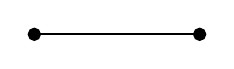
\begin{tikzpicture}[thick, scale=0.7]
    	\tikzstyle{point}=[circle,thick,draw=black,fill=black,inner sep=0pt,minimum width=4pt,minimum height=4pt]
    	\node (a)[point] at (0,0) {};
    	\node (b)[point] at (3,0) {};
 
    	\draw (a.center) -- (b.center) --cycle;
	\end{tikzpicture}
	\caption{1-símplice}\label{ref:1simp}
\end{subfigure}\hspace{0.05\textwidth}
\begin{subfigure}[b]{0.2\textwidth}
\centering
	\begin{tikzpicture}[thick, scale=3]
    	\tikzstyle{point}=[circle,thick,draw=black,fill=black,inner sep=0pt,minimum width=4pt,minimum height=4pt]
    	\coordinate (a) at (0,0);
    	\coordinate (b) at (1,0);
    	\coordinate (c) at (0.6,0.5);

    	\draw[fill=greeo,opacity=0.6] (a) -- (b) -- (c) -- cycle;
 
    	\draw (a) -- (b) -- (c)  --cycle;
    	
    	\node ()[point] at (a) {};
    	\node ()[point] at (b) {};
    	\node ()[point] at (c) {};
	\end{tikzpicture}
	\caption{2-símplice}\label{ref:2simp}
\end{subfigure}\hspace{0.05\textwidth}
\begin{subfigure}[b]{0.2\textwidth}
\centering
	\begin{tikzpicture}[thick,scale=3]
    	\tikzstyle{point}=[circle,thick,draw=black,fill=black,inner sep=0pt,minimum width=4pt,minimum height=4pt]

	\coordinate (A1) at (0,0);
	\coordinate (A3) at (1,0);
	\coordinate (A4) at (0.4,-0.3);
	\coordinate (B1) at (0.5,0.5);

	\draw[thick,dashed,opacity=0.6] (A1) -- (A3);
	\draw[fill=greeo,opacity=0.6] (A1) -- (A4) -- (B1) -- cycle;
	\draw[fill=greeo,opacity=0.6] (A3) -- (A4) -- (B1) -- cycle;

	\draw (A1) -- (B1)  -- (A3) -- (A4) --(A1) --cycle;
	
	\node ()[point] at (A1) {};
	\node ()[point] at (A3) {};
	\node ()[point] at (A4) {};
	\node ()[point] at (B1) {};
	\end{tikzpicture}
	\caption{3-símplice}\label{ref:3simp}
\end{subfigure}
\caption{Representación de los símplices de dimensión 0, 1, 2 y 3}
\end{figure}

Se puede observar que cualquier subconjunto de los vértices de $\sigma$ será afínmente independiente y por lo tanto definirá un símplice $\tau$. De esta forma diremos que \emph{$\tau$ es una cara de $\sigma$}  si es una combinación convexa de un subconjunto no vacío de los vértices de $\sigma$, y lo denotaremos por $\tau \leq \sigma$. Si el subconjunto es propio, diremos que \emph{$\tau$ es cara propia de $\sigma$}, y lo denotaremos por $\tau < \sigma$. Por otro lado, diremos que \emph{$\sigma$ es cocara (propia) de $\tau$}  si $\sigma \geq \tau$ ($\sigma > \tau$).

Haciendo uso de de la definición de caras de un símplice $\sigma$ podemos definir \emph{el borde y el interior} de $\sigma$.

\begin{definition}
Sea $\sigma$ un símplice. Entonces
\begin{itemize}
	\item Se define el \emph{borde de $\sigma$} como \[bd \ \sigma = \bigcup_{\tau<\sigma}\tau\]
	\item Se define el \emph{interior de $\sigma$} como \[int\ \sigma= \sigma - bd\ \sigma\]
\end{itemize}
\end{definition}

Debido a la definición del símplice como la envolvente convexa de un conjunto de puntos afínmente independientes, un punto $x \in \sigma$ pertenece al interior de $\sigma$ si y sólo si todos sus coeficientes $\lambda_i$ de la combinación convexa son positivos. Se sigue que cada punto $x \in \sigma$ pertenece únicamente al interior de la cara generada por los puntos con coeficientes $\lambda_i$ positivos.

Una vez que ya conocemos las piezas de nuestra descomposición vamos a ver como tenemos que unirlas y cuales son las principales propiedades de los complejos resultantes.\\
Como ya hemos visto al principio de la sección, para que una descomposición sea un complejo sus piezas tienen que ser topológicamente simples y sus intersecciones tienen que ser piezas de dimensión inferior del mismo tipo. Es por esto que la manera que tendremos que unir unos símplices con otros por sus caras.

\begin{definition}
Un \emph{complejo simplicial} es una colección finita de símplices $K$ que satisface las siguientes propiedades:
\begin{enumerate}
	\item Si $\sigma \in K$ y $\tau \leq \sigma$ entonces $\tau \in K$.
	\item Si $\sigma_0,\sigma_1 \in K$ y $\sigma_0 \cap \sigma_1 \neq \emptyset$ entonces $\sigma_0 \cap \sigma_1 \leq \sigma_i$ para $i = 1,2$.
\end{enumerate}
\end{definition}

Se define la dimensión de como el máximo de las dimensiones de sus símplices.

Un ejemplo de complejo simplicial es lo que se muestra en la figura \ref{ref:comp1}, mientras que en la figura \ref{ref:noComp} muestra un ejemplo que no es complejo simplicial.


\begin{figure}[ht]
\centering
\begin{tikzpicture}[thick,scale=3]
    	\tikzstyle{point}=[circle,thick,draw=black,fill=black,inner sep=0pt,minimum width=4pt,minimum height=4pt]

	\coordinate (x) at (0,0);

	\coordinate (A1) at (1,0);
	\coordinate (A3) at (2, 0.1);
	\coordinate (A4) at (1.4,-0.3);
	\coordinate (B1) at (1.5,0.5);

    \coordinate (b) at (3,0);
    \coordinate (c) at (2.6,-0.5);
    
    \coordinate (a1) at (3.4,0.12);
    \coordinate (b1) at (4,0);
    \coordinate (c1) at (3.8,0.3);
    
    \coordinate (y) at (3.5,-0.4);
	
	\draw[thick,dashed,opacity=0.6] (A1) -- (A3);
    \draw[fill=greeo,opacity=0.6] (a1) -- (b1) -- (c1) -- cycle;
	\draw[fill=greeo,opacity=0.6] (A1) -- (A4) -- (B1) -- cycle;
	\draw[fill=greeo,opacity=0.6] (A3) -- (A4) -- (B1) -- cycle;

	\draw (a1) -- (b1) -- (c1)  --cycle;	
	\draw (A1) -- (B1)  -- (A3) -- (A4) --(A1) --cycle;
	\draw (x) -- (A1) --cycle;	
	\draw (A3) -- (b) -- (c)  --cycle;	
	\draw (b1) -- (y) --cycle;
	\draw (B1) -- (A4) --cycle;
	
	\node ()[point] at (x) {};
	\node ()[point] at (A1) {};
	\node ()[point] at (A3) {};
	\node ()[point] at (A4) {};
	\node ()[point] at (B1) {};
    \node ()[point] at (b) {};
    \node ()[point] at (c) {};
    \node ()[point] at (a1) {};
    \node ()[point] at (b1) {};
    \node ()[point] at (c1) {};
    \node ()[point] at (y) {};	
	
	\end{tikzpicture}
\caption{Ejemplo de complejo simplicial}
\label{ref:comp1}
\end{figure}

\begin{figure}[ht]
\centering
\begin{tikzpicture}[thick]
    \tikzstyle{point}=[circle,thick,draw=black,fill=black,inner sep=0pt,minimum width=4pt,minimum height=4pt]
    \coordinate (a) at (0,0);
    \coordinate (b) at (3,0);
    \coordinate (c) at (2,2);

    \begin{scope}[yshift=2cm]
    	\coordinate (d) at (1,1);
    	\coordinate (e) at (0,2);
    	\coordinate (f) at (4,2);
    \end{scope}

	\coordinate (p) at (1.5,0.5);

    \draw[fill=greeo,opacity=0.6] (a) -- (b) -- (c) -- cycle;
    \draw[fill=greeo,opacity=0.6] (d) -- (e) -- (f) -- cycle;
    
 
    \draw (p) -- (d) --cycle;
    \draw (a) -- (b) -- (c)  --cycle;
    \draw (d) -- (e) -- (f) -- cycle;    
    
	\node ()[point] at (a) {};
    \node ()[point] at (b) {};
    \node ()[point] at (c) {};
    \node ()[point] at (d) {};
    \node ()[point] at (e) {};
    \node ()[point] at (f) {};
    \node ()[point] at (p) {};    
\end{tikzpicture}
\caption{Ejemplo de conjunto de símplices que no cumplen las condiciones de complejo simplicial}
\label{ref:noComp}
\end{figure}

El \emph{espacio subyacente} de un complejo simplicial $K$, denotado $\abs{K}$, es la unión de los símplices de $K$ con la topología heredada del $\mathbb{R}^d$ donde viven sus símplices. Este espacio subyacente también es llamado \emph{poliedro}. Como se puede observar, el espacio subyacente  de un complejo simplicial es compacto, el cual es un resultado que nos será necesario para la demostración del Teorema de Estabilidad.

Dada esta definición del espacio subyacente de un complejo simplicial podemos conocer cuales son los  subconjuntos abiertos y cerrados de $\abs{K}$.
\begin{proposition}
Sea $K$ un complejo simplicial y $A \subset \abs{K}$ un subconjunto. Entonces $A$ es un abierto (cerrado) en $K$ si y sólo si para cada $\sigma \in K$, $A \cap \abs{\sigma}$ es un abierto (cerrado) de $\abs{\sigma}$.
\end{proposition}

Una vez que conocemos como se definen los complejos simpliciales y su correspondiente topología, vamos a ver como vincular un espacio topológico con un complejo simplicial. Para ello haremos uso de las triangulaciones:

\begin{definition}
Una \emph{triangulación} de un espacio topológico $X$ es un par $(K, h)$ donde $K$ es un complejo simplicial y $h: X \longrightarrow \abs{K}$ es un homeomorfismo ($h$ continua, biyectiva y $h^{-1}$ continua).
\end{definition}
Diremos que un espacio topológico es \emph{triangulable} si admite una triangulación. Y por tanto, los espacios $\abs{K}$ y $X$ son iguales (topológicamente hablando).

También nos será de utilidad poder estudiar los complejos simpliciales contenidos en otro complejo simplicial.
\begin{definition}
Un \emph{subcomplejo} $L$ de un complejo simplicial $K$ es un complejo simplicial $L \subseteq K$.
\end{definition}

Un subcomplejo de gran interés son los \emph{$j$-esqueletos}, definidos de la siguiente forma: \[K^{(j)} = \{\sigma \in K \mid dim\ \sigma\ \leq j\}\]

Otro subconjunto de símplices que nos será de gran ayuda más adelante es la \emph{estrella de un símplice $\tau$}, la cual consiste de las cocaras de $\tau$, denotado por St $\tau$. Este conjunto no será siempre un complejo simplicial, así que se define la \emph{estrella cerrada} $\overline{\text{St}}\ \tau$ como el menor subcomplejo de $K$ que contiene a St $\tau$. Adicionalmente, se define el \emph{link} de $\tau$ como: $\text{Lk }\tau = \{v \in \overline{\text{St}}\ \tau \mid v \cap \tau = \emptyset\}$.

\subsubsection*{Complejos simpliciales abstractos}
Una vez que ya conocemos los complejos simpliciales desde el punto de vista geométrico, vamos a abordarlos desde un enfoque combinatorio, el cual nos será de gran ayuda para poder programar los complejos simpliciales.

\begin{definition}
Un \emph{complejo simplicial abstracto $A$} es una colección finita de conjuntos finitos tal que si $\alpha \in A$ y $\beta \subset \alpha$ entonces $\beta \in A$.
\end{definition}
De esta forma se cumple que
\begin{itemize}
	\item Los conjuntos en $A$ no vacíos se denominan \emph{símplices abstractos}.
	\item La \emph{dimensión} de un símplice abstracto $\alpha \in A$ es $dim\ \alpha = card(\alpha) - 1$. Y la dimensión del complejo es el máximo de las dimensiones de sus símplices.
	\item Una \emph{cara} de $\alpha \in A$ es cualquier subconjunto no vacío de $\beta \subset \alpha$.
	\item El \emph{conjunto de vértices} de $A$ es la unión de todos sus símplices.
	\item Un \emph{subcomplejo $B$} de un complejo simplicial abstracto $A$ es un complejo simplicial abstracto $B \subset A$.
\end{itemize}

\begin{exmp}
Un ejemplo de complejo simplicial abstracto es el siguiente conjunto 

\begin{gather*}
A = \{\{0\},\{1\},\{2\},\{3\},\{4\},\{5\},\{6\},\{0,1\},\{1,2\},\{1,3\},\{1,4\},\{2,3\},\{2,4\},\{3,4\},\{4,5\},\\
\{4,6\},\{5,6\},\{1,2,3\},\{1,2,4\},\{1,3,4\},\{2,3,4\},\{1,2,3,4\}\}
\end{gather*}

Donde el conjunto de vértices es: $Vert\ A = \{0, 1, 2, 3, 4, 5, 6\}$.
\end{exmp}

\begin{definition}
Sean $A$ y $B$ dos complejos simpliciales abstractos. Diremos que $A$ y $B$ son \emph{isomorfos} si existe una biyección \[b:Vert\ A \longrightarrow Vert\ B\] tal que $\alpha \in A$ si y sólo si $b(\alpha) \in B$.
\end{definition}
De esta forma podremos ver si varios complejos simpliciales abstractos realmente representan el mismo complejo abstracto. Sin embargo, lo que más nos interesaría es ver si un complejo simplicial abstracto puede representar correctamente un complejo simplicial (definido geométricamente) y viceversa. 

Siempre podremos generar complejos simpliciales abstractos a partir de un complejo simplicial (geométrico) de la siguiente forma:
\begin{definition}
Sea $K$ un complejo simplicial y $V$ el conjunto de vértices de $K$. Llamaremos \emph{esquema de vértices} al complejo simplicial abstracto $A$ formado por todos aquellos subconjuntos de $V$ que generan símplices en $K$.
\end{definition}

Y bajo ciertas cirscunstancias podremos hacer el paso opuesto de construir un complejo simplicial (geométrico) a partir de otro abstracto:
\begin{definition}
Sean $A$ un complejo simplicial abstracto y $K$ un complejo simplicial. Diremos que $K$ es una \emph{realización geométrica} de $A$, si $A$ es isomorfo al esquema de vértices de $K$.
\end{definition}

\begin{theorem}
Todo complejo simplicial abstracto de dimensión $d$ admite una realización geométrica en $\mathbb{R}^{2d + 1}$.
\end{theorem}

Así pues, garantizamos los complejos simpliciales abstractos como una representación fiel de un complejo simplicial (geométrico).

\subsubsection*{Aplicaciones simpliciales}
Una vez que ya conocemos las principales propiedades de los complejos simpliciales, veremos como podemos definir aplicaciones continuas entre ellos. Como vimos anteriormente, para todo $\sigma$ cada punto de un $k$-símplice pertenece al interior de exactamente una cara. Por lo tanto, todo punto $x \in \abs{K}$, siendo $K$ un complejo simplicial de vértices $u_0, u_1, ..., u_n$, pertenece al interior de uno de los símplices de $K$. Si $\sigma = conv\{u_0, u_1, ..., u_k\}$ es dicho símplice, entonces $x = \sum_{i=0}^{n} b_i(x)u_i$, donde
\[
b_i(x)=
\begin{cases}
\lambda_i	 & \text{ si } 0 \leq i \leq k \\ 
0 			 & \text{ si } k+1 \leq i \leq n
\end{cases},\text{ con } \lambda_i \text{ tal que } x = \sum_{i=0}^{k} \lambda_i u_i
\]
son las \emph{coordenadas baricéntricas} de x en $K$.

Haremos uso de estas coordenadas para construir una función continua, lineal a trozos inducida por una función entre los vértices de dos complejos simpliciales, denominada \emph{aplicación de vértices}

\begin{definition}
Sean $K$ y $L$ complejos simpliciales y $\varphi:\text{Vert }K \longrightarrow \text{Vert }L$ una aplicación. Diremos que $\varphi$ es una \emph{aplicación de vértices} si satisface que para cada $\sigma \in K$ su imagen $\varphi(\sigma) \in L$.
\end{definition}

Una aplicación de vértices $\varphi:\text{Vert }K \longrightarrow \text{Vert }L$ induce una aplicación continua, lineal a trozos $f: \abs{K} \longrightarrow \abs{L}$ dada por
\[
f(x) = f\left ( \sum_{i=0}^{n} b_i(x) u_i \right ) =  \sum_{i=0}^{n} b_i(x)u_i
\]
a la que llamaremos \emph{aplicación simplicial} asociada a $\varphi$. Para enfatizar que es una aplicación lineal en cada símplice del complejo, se suele notar la aplicación de la siguiente forma $f: K \longrightarrow L$. 

\subsubsection*{Subdivisiones}
Veremos que hay ocasiones que nos interesará poder ir haciendo los símplices de nuestro complejo simplicial más pequeños, pero conservando el espacio topológico. Por esta razón, definimos \emph{subdivisión de un complejo simplicial} de la siguiente manera:
\begin{definition}
Sea $K$ un complejo simplicial. Diremos que un complejo simplicial $L$ es una \emph{subdivisión} de $K$ si:
\begin{itemize}
	\item $\abs{K}=\abs{L}$.
	\item Cada símplice de $L$ está contenido en un símplice de $K$.
\end{itemize}
\end{definition}

Hay muchas maneras de obtener subdivisiones de un complejo simplicial, pero nosotros nos centraremos en la \emph{subdivisión baricéntrica}, denotado por $L =$ Sd$K$. Para la construcción de esta subdivisión, tenemos que definir el \emph{baricentro} de un símplice y el \emph{cono} de un símplice de vértice $v$.

\begin{definition}
Sea $\sigma$ un $k$-símplice, tal que $\sigma = conv\{v_0, v_1, ..., v_k\}$. Llamaremos \emph{baricentro} de $\sigma$ al punto
\[
b_\sigma = \sum_{i=0}^{k} \frac{v_i}{k+1}\ \in int\ \sigma
\]
\end{definition}

\begin{definition}
Sea $\sigma$ un $k$-símplice, tal que $\sigma = conv\{v_0, v_1, ..., v_k\}$ y $v$ un punto no contenido en el subespacio afín generado por $\{v_0, v_1, ..., v_k\}$. Se define el \emph{cono} de $\sigma$ con vértice $v$ y se denota por $\sigma*v$ como el $k+1$-símplice generado por $\{v,v_0, v_1, ..., v_k\}$.
\end{definition}

Sea $K$ un complejo simplicial. Se define la \emph{subdivisión baricéntrica} de $K$ como el complejo simplicial Sd$K$ que se construye inductivamente sobre el $j$-esqueleto como sigue:
\begin{enumerate}
	\item Sd$K^{(0)} = K^{(0)}$.
	\item Sd$K^{(j)}$ es la unión de Sd$K^{(j-1)}$ con el conjunto de todos los símplices de la forma $b_\sigma*\tau$, donde $\sigma$ es un $j$-símplice y $\tau$ es cualquier símplice de Sd$K^{(j-1)}$ contenido en una cara de $\sigma$.
\end{enumerate}
En la figura \ref{ref:subBar} se muestra la primera y segunda subdivisión baricéntrica de un complejo simplicial.

\begin{figure}[h]
\centering
\begin{subfigure}[b]{0.3\textwidth}
\centering
	\begin{tikzpicture}[thick, scale=4]
    	\tikzstyle{point0}=[circle,thick,draw=black,fill=black,inner sep=0pt,minimum width=4pt,minimum height=4pt]
    	
    	\coordinate (a) at (0,0);
    	\coordinate (b) at (1,0);
    	\coordinate (c) at (0.5,0.7);

    	\draw[fill=greeo,opacity=0.6] (a) -- (b) -- (c) -- cycle;
 
    	\draw (a) -- (b) -- (c)  --cycle;
    	
    	\node ()[point0] at (a) {};
    	\node ()[point0] at (b) {};
    	\node ()[point0] at (c) {};
	\end{tikzpicture}
	\caption{2-símplice}\label{ref:2simpBar}
\end{subfigure}\hspace{0.02\textwidth}
\begin{subfigure}[b]{0.3\textwidth}
\centering
	\begin{tikzpicture}[thick, scale=4]
    	\tikzstyle{point0}=[circle,thick,draw=black,fill=black,inner sep=0pt,minimum width=4pt,minimum height=4pt]
    	\tikzstyle{point1}=[circle,thick,draw=black,fill=red,inner sep=0pt,minimum width=4pt,minimum height=4pt]
    	
    	\coordinate (a) at (0,0);
    	\coordinate (b) at (1,0);
    	\coordinate (c) at (0.5,0.7);
    	\coordinate (d) at (0.25,0.35);
    	\coordinate (e) at (0.5,0);
    	\coordinate (f) at (0.75,0.35);
    	\coordinate (g) at (0.5,0.23);

		\draw[fill=greeo,opacity=0.6] (a) -- (b) -- (c) -- cycle;
		
    	\draw (a) -- (b) -- (c)  --cycle;
    	\draw (a) -- (f) --cycle;
    	\draw (c) -- (e) --cycle;
    	\draw (d) -- (b) --cycle;
    	
		\node ()[point0] at (a) {};
		\node ()[point0] at (b) {};
		\node ()[point0] at (c) {};   
    	\node ()[point1] at (d) {};
    	\node ()[point1] at (e) {};
    	\node ()[point1] at (f) {};
    	\node ()[point1] at (e) {};
    	\node ()[point1] at (g) {};
	\end{tikzpicture}
	\caption{Primera subdivisión baricéntrica}\label{ref:1SubBar}
\end{subfigure}\hspace{0.02\textwidth}
\begin{subfigure}[b]{0.3\textwidth}
\centering
	\begin{tikzpicture}[thick, scale=4]
    	\tikzstyle{point0}=[circle,thick,draw=black,fill=black,inner sep=0pt,minimum width=4pt,minimum height=4pt]
    	\tikzstyle{point1}=[circle,thick,draw=black,fill=red,inner sep=0pt,minimum width=4pt,minimum height=4pt]
    	\tikzstyle{point2}=[circle,thick,draw=black,fill=blue,inner sep=0pt,minimum width=4pt,minimum height=4pt]
    	
    	\coordinate (a) at (0,0);
    	\coordinate (b) at (1,0);
    	\coordinate (c) at (0.5,0.7);
    	\coordinate (d) at (0.25,0.35);
    	\coordinate (e) at (0.5,0);
    	\coordinate (f) at (0.75,0.35);
    	\coordinate (g) at (0.5,0.23);
    	\coordinate (h) at (0.38,0.53);
    	\coordinate (i) at (0.5,0.47);
    	\coordinate (j) at (0.63,0.53);
    	\coordinate (k) at (0.38,0.29);
    	\coordinate (l) at (0.63,0.29);
    	\coordinate (m) at (0.42,0.43);
    	\coordinate (n) at (0.58,0.43);
    	\coordinate (o) at (0.13,0.18);
    	\coordinate (p) at (0.25,0.12);
    	\coordinate (q) at (0.5,0.12);
    	\coordinate (r) at (0.25,0);
    	\coordinate (s) at (0.25,0.19);
    	\coordinate (t) at (0.33,0.08);
    	\coordinate (u) at (0.88,0.18);
    	\coordinate (v) at (0.75,0.12);
    	\coordinate (w) at (0.75,0);
    	\coordinate (x) at (0.67,0.08);
    	\coordinate (y) at (0.75,0.19);

		\draw[fill=greeo,opacity=0.6] (a) -- (b) -- (c) -- cycle;
		
    	\draw (a) -- (b) -- (c)  --cycle;
    	\draw (a) -- (f) --cycle;
    	\draw (c) -- (e) --cycle;
    	\draw (d) -- (b) --cycle;
    	\draw (c) -- (k) --cycle;
    	\draw (g) -- (h) --cycle;
    	\draw (d) -- (i) --cycle;
    	\draw (c) -- (l) --cycle;
    	\draw (g) -- (j) --cycle;
    	\draw (f) -- (i) --cycle;
    	\draw (a) -- (k) --cycle;
    	\draw (d) -- (p) --cycle;
    	\draw (g) -- (o) --cycle;
    	\draw (g) -- (r) --cycle;
    	\draw (e) -- (p) --cycle;
    	\draw (a) -- (q) --cycle;
    	\draw (e) -- (v) --cycle;
    	\draw (b) -- (q) --cycle;
    	\draw (g) -- (w) --cycle;
    	\draw (b) -- (l) --cycle;
    	\draw (g) -- (u) --cycle;
    	\draw (f) -- (v) --cycle;
    	
		\node ()[point0] at (a) {};
		\node ()[point0] at (b) {};
		\node ()[point0] at (c) {};   
    	\node ()[point1] at (d) {};
    	\node ()[point1] at (e) {};
    	\node ()[point1] at (f) {};
    	\node ()[point1] at (e) {};
    	\node ()[point1] at (g) {};
    	\node ()[point1] at (f) {};
    	\node ()[point1] at (g) {};
    	\node ()[point2] at (h) {};
    	\node ()[point2] at (i) {};
    	\node ()[point2] at (j) {};
    	\node ()[point2] at (k) {};
    	\node ()[point2] at (l) {};
    	\node ()[point2] at (m) {};
    	\node ()[point2] at (n) {};
    	\node ()[point2] at (o) {};
    	\node ()[point2] at (p) {};
    	\node ()[point2] at (q) {};
    	\node ()[point2] at (r) {};
    	\node ()[point2] at (s) {};
    	\node ()[point2] at (t) {};
    	\node ()[point2] at (u) {};
    	\node ()[point2] at (v) {};
    	\node ()[point2] at (w) {};
    	\node ()[point2] at (x) {};
    	\node ()[point2] at (y) {};
	\end{tikzpicture}
	\caption{Segunda subdivisión baricéntrica}\label{ref:2SubBar}
\end{subfigure}
\caption{Primera y segunda subdivisión baricéntrica de un 2-símplice}
\label{ref:subBar}
\end{figure}

Recordemos que el \emph{diámetro} de un subconjunto $A \subset \mathbb{R}^d$ es el supremo sobre las distancias entre sus puntos. 

\begin{lemma}
Si $\sigma$ es un $k$-símplice, entonces el diámetro de cada símplice en la subdivisión baricéntrica de $\sigma$ es como máximo $\frac{k}{k+1}diam\ \sigma$. 
\end{lemma}

De forma que gracias al lema anterior podremos hacer el diámetro de los símplices de los complejos simpliciales tanto como queramos, ya que el diámetro de los símplices de la n-ésima subdivisión baricéntrica del complejo simplicial $K$, denotado por Sd$^nK =$ Sd(Sd$^{n - 1}K$), es 
\[
\left ( \frac{k}{k+1} \right )^n diam\ \sigma  \underset{n \to \infty}{\longrightarrow} 0,\ con\ \sigma \in K 
\]

\subsubsection*{Aproximaciones simpliciales}
También nos es de interés poder aproximar funciones continuas entre los subespacios subyacentes de dos complejos simpliciales a partir de una aplicación simplicial entre dichos complejos. Para poder definir esta aproximación primero vamos a definir un tipo de entorno de los vértices de un complejo como se puede ver en la figura \ref{ref:entEstrellado}.

\begin{definition}
Sea $K$ un complejo simplicial y $v$ un vértice de $K$. El conjunto
\[
N(v) = \bigcup_{\sigma \in \text{St } v} int\ \sigma
\]
es un entorno abierto de $v$ en $\abs{K}$ al que llamaremos \emph{entorno estrellado} de $v$.
\end{definition}

\begin{figure}[h]
\centering
	\begin{tikzpicture}[thick, scale=4]
    	\tikzstyle{point}=[circle,thick,draw=black,fill=black,inner sep=0pt,minimum width=4pt,minimum height=4pt]

    	
    	\coordinate (a) at (0,0);
    	\coordinate (b) at (1,0);
    	\coordinate (c) at (0.5,0);
    	\coordinate (d) at (0.5,0.5);
    	\coordinate (e) at (0.5,-0.5);
    	\coordinate (f) at (1.29,0.44);
    	\coordinate (g) at (1.5,-0.49);
    	\coordinate (h) at (1.02,-0.64);
    	
		\node ()[point] at (c) {};		
		
		\draw[fill=greeo,opacity=0.6] (e) -- (h) -- (g) -- (f) -- (d) -- (b) -- cycle;
				
    	\draw (a) -- (d) -- (f)  -- (g) -- (h) -- (e) --cycle;
    	\draw (a) -- (b) --cycle;
    	\draw (d) -- (e) --cycle;
    	\draw (b) -- (f) --cycle;
    	\draw (b) -- (g) --cycle;
    	\draw (b) -- (h) --cycle;
    
    	\draw[fill=redp,opacity=0.6] (a) -- (d) -- (b) -- (e) -- cycle;
    	
		\node ()[point] at (a) {};
		\node ()[point] at (b) {};
		\node ()[label={[shift={(0.2,-0.15)}]\small $v$}] at (c) {};
    	\node ()[point] at (d) {};
    	\node ()[point] at (e) {};
    	\node ()[point] at (f) {};
    	\node ()[point] at (e) {};
    	\node ()[point] at (g) {};
    	\node ()[point] at (h) {};
    	\node () at (0.35,0.17) {$N(v)$};
	\end{tikzpicture}
\caption{Entorno estrellado de $v$ marcado en color rojo}
\label{ref:entEstrellado}
\end{figure}

Así pues, definimos una aproximación simplicial de la siguiente forma:
\begin{definition}
Sean $K$ y $L$ complejos simpliciales, $g: \abs{K} \longrightarrow \abs{L}$ una aplicación continua y  $f: K \longrightarrow L$ una aplicación simplicial. Diremos que $f$ es una \emph{aproximación simplicial} de $g$ si verifica la \emph{condición de estrella}, es decir, si para cada vértice $v \in K$ se tiene que $g(N(v)) \subset N(f(v))$.
\end{definition}

Además la condición de estrella será una condición suficiente para garantizar la existencia de una aproximación simplicial:
\begin{lemma}
Sean $K$ y $L$ complejos simpliciales, $g: \abs{K} \longrightarrow \abs{L}$ una aplicación continua que satisface la condición de estrella. Entonces $g$ tiene una aproximación simplicial $f: K \longrightarrow L$.
\end{lemma}

%TODO METER RELLENO
\begin{theorem}[Aproximación simplicial]
\label{ref:teoremaAproximacionSimplicial}
\begin{sloppypar}
Sean $K$ y $L$ complejos simpliciales, ${g: \abs{K} \longrightarrow \abs{L}}$ una aplicación continua. Entonces existe $n \in \mathbb{N}$ tal que $g$ tiene una aproximación simplicial ${f: \textit{Sd}^{n}\ K \longrightarrow L}$.
\end{sloppypar}
\end{theorem}

\subsubsection*{Complejos simpliciales de nubes de puntos}
Desde el punto de vista computacional nos encontramos con el problema de que tenemos una representación de un espacio topológico a través de una discretización finita de los puntos de dicho espacio, y nuestro objetivo es poder recuperar las propiedades del espacio topológico original a partir de esta nube de puntos. Para ello usaremos complejos simpliciales asociados a dicha nube de puntos.

\subsubsection*{def complejo de \v{C}ech}
\subsubsection*{def complejo de Vietoris-Rips}
\subsubsection*{def diagrama de Voronoi + triangulación Delonay}
\subsubsection*{def alpha complejo}

\subsection{Homología}
Como se puede ver en [añadir cita] la homotopía es una gran herramienta algebraica para poder obtener propiedades de los espacios topológicos. Sin embargo, los métodos para el cálculo de la homotopía no son los mejores computacionalmente. Así pues, se propone la homología como formalismo algebraico, que aunque no es capaz de obtener tanta información topológica sobre el espacio como con otros formalismos, contiene algoritmos mucho más rápidos y eficientes.

Comenzaremos estudiando los diversos grupos que están involucrados en la definición de la homología.

\subsubsection*{Grupos de cadenas}
Sea $K$ un complejo simplicial y $p$ un número entero no negativo. Una \emph{$p$-cadena} en $K$ es una suma formal de $p$-símplices en $K$. Más concretamente, $c$ es una $p$-cadena en $K$ si
\[
c = \sum a_i\sigma_i
\]
con $\sigma_i$ es un $p$-símplice para cada $i$ y $a_i$ son los \emph{coeficientes}. Estos coeficientes pueden tomarse de cualquier anillo conmutativo, sin embargo, nosotros usaremos con coeficientes de módulo 2, es decir, $a_i \in \mathbb{Z}_2$. 

\begin{exmp}
Escribiremos los símplices como la lista de sus vértices, $\sigma = [u_0, u_1, ..., u_p]$.
\begin{itemize}
	\item En la figura \ref{ref:0cad} se muestra en rojo la $0$-cadena $c=[0]+[2]+[6]+[9]$.
\begin{figure}[!ht]
\centering
\begin{tikzpicture}[thick,scale=3]
    	\tikzstyle{point}=[circle,thick,draw=black,fill=black,inner sep=0pt,minimum width=4pt,minimum height=4pt]
    	\tikzstyle{point1}=[circle,thick,draw=black,fill=red,inner sep=0pt,minimum width=7pt,minimum height=7pt]

	\coordinate (x) at (0,0);

	\coordinate (A1) at (1,0);
	\coordinate (A3) at (2, 0.1);
	\coordinate (A4) at (1.4,-0.3);
	\coordinate (B1) at (1.5,0.5);

    \coordinate (b) at (3,0);
    \coordinate (c) at (2.6,-0.5);
    
    \coordinate (a1) at (3.4,0.12);
    \coordinate (b1) at (4,0);
    \coordinate (c1) at (3.6,0.3);
    
    \coordinate (y) at (3.5,-0.4);
	
	\draw[thick,dashed,opacity=0.6] (A1) -- (A3);
    \draw[fill=greeo,opacity=0.6] (b) -- (b1) -- (c1) -- cycle;
	\draw[fill=greeo,opacity=0.6] (A1) -- (A4) -- (B1) -- cycle;
	\draw[fill=greeo,opacity=0.6] (A3) -- (A4) -- (B1) -- cycle;

	\draw (b) -- (b1) -- (c1)  --cycle;	
	\draw (A1) -- (B1)  -- (A3) -- (A4) --(A1) --cycle;
	\draw (x) -- (A1) --cycle;	
	\draw (A3) -- (b) -- (c)  --cycle;	
	\draw (b1) -- (y) --cycle;
	\draw (B1) -- (A4) --cycle;	
	
	\node ()[point1,label={$0$}] at (x) {};
	\node ()[point,label={$1$}] at (A1) {};
	\node ()[point1,label={$2$}] at (B1) {};
	\node ()[point,label={[shift={(0.3,-0.5)}]$3$}] at (A4) {};
	\node ()[point,label={$4$}] at (A3) {};
	\node ()[point,label={$5$}] at (c) {};
    \node ()[point1,label={$6$}] at (b) {};
    \node ()[point,label={$7$}] at (c1) {};
    \node ()[point,label={$8$}] at (b1) {};
    \node ()[point1,label={$9$}] at (y) {};	
	
	\end{tikzpicture}
\caption{Ejemplo de $0$-cadena}
\label{ref:0cad}
\end{figure}
	\item En la figura \ref{ref:1cad} se muestra en rojo la $1$-cadena $c=[0,1]+[1,2]+[2,4]+[8,9]$.
\begin{figure}[!ht]
\centering
\begin{tikzpicture}[thick,scale=3]
    	\tikzstyle{point}=[circle,thick,draw=black,fill=black,inner sep=0pt,minimum width=4pt,minimum height=4pt]
    	\tikzstyle{point1}=[circle,thick,draw=black,fill=red,inner sep=0pt,minimum width=7pt,minimum height=7pt]
    	\tikzstyle{line}=[line width=1.5pt, red]

	\coordinate (x) at (0,0);

	\coordinate (A1) at (1,0);
	\coordinate (A3) at (2, 0.1);
	\coordinate (A4) at (1.4,-0.3);
	\coordinate (B1) at (1.5,0.5);

    \coordinate (b) at (3,0);
    \coordinate (c) at (2.6,-0.5);
    
    \coordinate (a1) at (3.4,0.12);
    \coordinate (b1) at (4,0);
    \coordinate (c1) at (3.6,0.3);
    
    \coordinate (y) at (3.5,-0.4);
	
	\draw[thick,dashed,opacity=0.6] (A1) -- (A3);
    \draw[fill=greeo,opacity=0.6] (b) -- (b1) -- (c1) -- cycle;
	\draw[fill=greeo,opacity=0.6] (A1) -- (A4) -- (B1) -- cycle;
	\draw[fill=greeo,opacity=0.6] (A3) -- (A4) -- (B1) -- cycle;

	\draw (b) -- (b1) -- (c1)  --cycle;	
	\draw (A1) -- (B1)  -- (A3) -- (A4) --(A1) --cycle;
	\draw (A3) -- (b) -- (c)  --cycle;	
	\draw[line] (b1) -- (y) --cycle;
	\draw[line] (x) -- (A1) -- (B1) -- (A3);	
	\draw (B1) -- (A4) --cycle;
	
	\node ()[point1,label={$0$}] at (x) {};
	\node ()[point1,label={$1$}] at (A1) {};
	\node ()[point1,label={$2$}] at (B1) {};
	\node ()[point,label={[shift={(0.3,-0.5)}]$3$}] at (A4) {};
	\node ()[point1,label={$4$}] at (A3) {};
	\node ()[point,label={$5$}] at (c) {};
    \node ()[point,label={$6$}] at (b) {};
    \node ()[point,label={$7$}] at (c1) {};
    \node ()[point1,label={$8$}] at (b1) {};
    \node ()[point1,label={$9$}] at (y) {};	
	
	\end{tikzpicture}
\caption{Ejemplo de $1$-cadena}
\label{ref:1cad}
\end{figure}
	\item En la figura \ref{ref:2cad} se muestra en rojo la $2$-cadena $c=[1,2,3] + [2,3,4] + [6,7,8]$.
\begin{figure}[!ht]
\centering
\begin{tikzpicture}[thick,scale=3]
    	\tikzstyle{point}=[circle,thick,draw=black,fill=black,inner sep=0pt,minimum width=4pt,minimum height=4pt]
    	\tikzstyle{point1}=[circle,thick,draw=black,fill=red,inner sep=0pt,minimum width=7pt,minimum height=7pt]
    	\tikzstyle{line}=[line width=1.5pt, red]
    	
	\coordinate (x) at (0,0);

	\coordinate (A1) at (1,0);
	\coordinate (A3) at (2, 0.1);
	\coordinate (A4) at (1.4,-0.3);
	\coordinate (B1) at (1.5,0.5);

    \coordinate (b) at (3,0);
    \coordinate (c) at (2.6,-0.5);
    
    \coordinate (a1) at (3.4,0.12);
    \coordinate (b1) at (4,0);
    \coordinate (c1) at (3.6,0.3);
    
    \coordinate (y) at (3.5,-0.4);
	
	\draw[thick,dashed,opacity=0.6,line] (A1) -- (A3);
    \draw[fill=redp,opacity=0.6] (b) -- (b1) -- (c1) -- cycle;
	\draw[fill=redp,opacity=0.6] (A1) -- (A4) -- (B1) -- cycle;
	\draw[fill=redp,opacity=0.6] (A3) -- (A4) -- (B1) -- cycle;

	\draw[line] (b) -- (b1) -- (c1)  --cycle;	
	\draw[line] (A1) -- (B1)  -- (A3) -- (A4) --(A1) --cycle;
	\draw (x) -- (A1) --cycle;	
	\draw (A3) -- (b) -- (c)  --cycle;	
	\draw (b1) -- (y) --cycle;
	\draw[line] (B1) -- (A4) --cycle;

	
	\node ()[point,label={$0$}] at (x) {};
	\node ()[point1,label={$1$}] at (A1) {};
	\node ()[point1,label={$2$}] at (B1) {};
	\node ()[point1,label={[shift={(0.3,-0.5)}]$3$}] at (A4) {};
	\node ()[point1,label={$4$}] at (A3) {};
	\node ()[point,label={$5$}] at (c) {};
    \node ()[point1,label={$6$}] at (b) {};
    \node ()[point1,label={$7$}] at (c1) {};
    \node ()[point1,label={$8$}] at (b1) {};
    \node ()[point,label={$9$}] at (y) {};	
	
	\end{tikzpicture}
\caption{Ejemplo de $2$-cadena}
\label{ref:2cad}
\end{figure}
\end{itemize}
\end{exmp}


Dadas dos $p$-cadenas $c = \sum a_i\sigma_i$ y $c' = \sum b_i\sigma_i$, se define su suma como
\[
c + c' = \sum (a_i + b_i)\sigma_i
\]
Las $p$-cadenas con la operación suma $+$ forman el \emph{grupo de $p$-cadenas} denotado por $(C_p,+)$, pero como la operación se sobrentiende, se suele nombrar como $C_p=C_p(K)$.

Este grupo es un grupo abeliano, y como en nuestro caso los coeficientes están en $\mathbb{Z}_2$ también será $C_p(K)$ un espacio vectorial sobre $\mathbb{Z}_2$. Luego, fijado $p \in \mathbb{Z}$, una base del espacio vectorial $C_p(K)$ es el conjunto $\{\sigma_i^p \mid i=1,...,s_p\}$ formado por los símplices de dimensión $p$ de $K$. Como consecuencia $C_p(K)=\{0\}$, siendo $0 = \sum 0\sigma_i$, si $p < 0$ ó $p > \text{dim}(K)$.

\subsubsection*{Operador borde}
Para poder relacionar estos grupos definiremos el \emph{operador borde}, así pues, partiremos con la definición del borde de un símplice.

\begin{definition}
Sea $p$ un número entero y $\sigma \in K$ un $p$-símplice $\sigma = [v_0, v_1, ..., v_p]$ se define su \emph{borde} como la suma formal de sus caras $(p-1)$-dimensionales, es decir, 
\[
\partial_p\sigma = \sum_{j=0}^{p}[v_0, ..., \hat{v}_j, ..., v_p]
\]
donde $\hat{v}_j$ denota que $v_j$ se omite.
\end{definition}

En general, dada una $p$-cadena $c =\sum a_i\sigma_i$, se define su borde mediante la extensión lineal como  $\partial_p c= \sum_{j=0}^{p} a_i \partial_p \sigma_i$. Como consecuencia, el borde define una aplicación lineal $\partial_p: C_p \longrightarrow C_{p-1}$ entre grupos de cadenas denominada \emph{operador borde}. Para simplificar la notación suele omitirse el subíndice $p$ del operador borde, ya que siempre coincide con la dimensión de la cadena a la que se le aplica.

\begin{exmp}
Sea la $2$-cadena $c = [0,1] + [4,5]$, entonces el borde de $c$ es:
\[
\partial c = \partial [0,1] + \partial [4,5] = [0] + [1] + [4] + [5]
\]
\end{exmp}

Además, podemos definir el \emph{complejo de cadenas} asociado a un complejo simplicial $K$ como la sucesión de grupos de cadenas conectados por los operadores borde
\[
...\overset{\partial_{p+2}}{\longrightarrow}C_{p+1}\overset{\partial_{p+1}}{\longrightarrow}C_{p}\overset{\partial_{p}}{\longrightarrow}C_{p-1}\overset{\partial_{p-1}}{\longrightarrow}...
\]

\subsubsection*{Ciclos y bordes}
Distinguiremos dos tipos de cadenas, las cuales usaremos para poder definir los grupos de homología. 
\begin{definition}
Diremos que una $p$-cadena $c$ es un \emph{$p$-ciclo} si
\[
\partial c = 0
\]
o, equivalentemente, si $c \in \text{ker }\partial$.
\end{definition}

Debido a que $\partial$ conmuta con la suma $+$, el conjunto de $p$-ciclos $Z_p = \text{ker }\partial_p$ es un subgrupo (subespacio vectorial en nuestro caso) de $C_p$.

\begin{exmp}
Veremos que geométricamente los $p$-ciclos representan ciclos en el complejo simplicial. Estos a su vez pueden ser agujeros de dimensión $p$. En la figura \ref{ref:1-ciclo} se muestra en rojo el $1$-ciclo $[4,5] + [4,6] + [5,6]$, el cual es un agujero. Mientras que en azul se representa el  $1$-ciclo $[6,7] + [6,8] + [7,8]$, que no es un agujero.

\begin{figure}[!ht]
\centering
\begin{tikzpicture}[thick,scale=3]
    	\tikzstyle{point}=[circle,thick,draw=black,fill=black,inner sep=0pt,minimum width=4pt,minimum height=4pt]
    	\tikzstyle{point1}=[circle,thick,draw=black,fill=red,inner sep=0pt,minimum width=7pt,minimum height=7pt]
    	\tikzstyle{point2}=[circle,thick,draw=black,fill=blue,inner sep=0pt,minimum width=7pt,minimum height=7pt]
    	\tikzstyle{line}=[line width=1.5pt, red]
    	\tikzstyle{line1}=[line width=1.5pt, blue]

	\coordinate (x) at (0,0);

	\coordinate (A1) at (1,0);
	\coordinate (A3) at (2, 0.1);
	\coordinate (A4) at (1.4,-0.3);
	\coordinate (B1) at (1.5,0.5);

    \coordinate (b) at (3,0);
    \coordinate (c) at (2.6,-0.5);
    
    \coordinate (a1) at (3.4,0.12);
    \coordinate (b1) at (4,0);
    \coordinate (c1) at (3.6,0.3);
    
    \coordinate (y) at (3.5,-0.4);
	
	\draw[thick,dashed,opacity=0.6] (A1) -- (A3);
    \draw[fill=greeo,opacity=0.6] (b) -- (b1) -- (c1) -- cycle;
	\draw[fill=greeo,opacity=0.6] (A1) -- (A4) -- (B1) -- cycle;
	\draw[fill=greeo,opacity=0.6] (A3) -- (A4) -- (B1) -- cycle;

	\draw (b) -- (b1) -- (c1)  --cycle;	
	\draw (B1) -- (A3) -- (A4);
	\draw[line1] (A1) -- (B1) -- (A4) --cycle;
	\draw[line] (A3) -- (b) -- (c)  --cycle;	
	\draw (b1) -- (y) --cycle;
	\draw (x) -- (A1);	

	
	\node ()[point,label={$0$}] at (x) {};
	\node ()[point2,label={$1$}] at (A1) {};
	\node ()[point2,label={$2$}] at (B1) {};
	\node ()[point2,label={[shift={(0.3,-0.5)}]$3$}] at (A4) {};
	\node ()[point1,label={$4$}] at (A3) {};
	\node ()[point1,label={$5$}] at (c) {};
    \node ()[point1,label={$6$}] at (b) {};
    \node ()[point,label={$7$}] at (c1) {};
    \node ()[point,label={$8$}] at (b1) {};
    \node ()[point,label={$9$}] at (y) {};	
	
	\end{tikzpicture}
\caption{Ejemplos de $1$-ciclos}
\label{ref:1-ciclo}
\end{figure}
\end{exmp}


\begin{definition}
\begin{sloppypar}
Diremos que una $p$-cadena $c$ es un \emph{$p$-borde} si existe una ${(p+1)\text{-cadena}}$ $c'$ tal que
\[
\partial c' = c
\]
o, equivalentemente, si $c \in \text{im }\partial_{p+1}$.
\end{sloppypar}
\end{definition}

Debido a que $\partial$ conmuta con la suma $+$, el conjunto de $p$-bordes $B_p = \text{im }\partial_{p+1}$ es un subgrupo (subespacio vectorial en nuestro caso) de $C_p$.

\begin{exmp}
El $1$-ciclo que habíamos destacado en azul en la figura \ref{ref:1-ciclo} es un $1$-borde.
\end{exmp}

Probaremos que los $p$-bordes son $p$-ciclos, como ocurre en el ejemplo. Para ello enunciaremos el siguiente lema.

\begin{lemma}[Lema fundamental de la homología]
$\partial_p \partial_{p+1} c = 0$ para todo entero $p$ y toda $(p + 1)$-cadena $c$.
\end{lemma}

Se sigue que $B_p$ es un subgrupo (en nuetro caso subespacio vectorial) de $Z_p$, es decir $B_p \subset Z_p$. La figura \ref{ref:gruposCadenasOpBorde} muestra esta relación entre el grupo de cadenas $C_p$, el grupo de ciclos $Z_p$ y el grupo de bordes $B_p$; y sus conexiones generadas por el operador borde.

\begin{figure}[!ht]
\centering
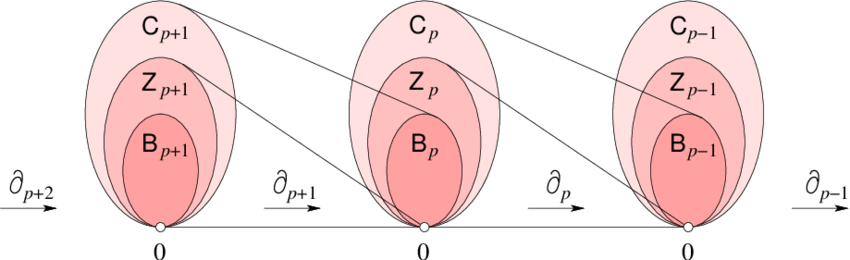
\includegraphics[width=0.8\textwidth]{include/figuras/The-chain-complex-consisting-of-a-linear-sequence-of-chain-cycle-and-boundary-groups.png} 
\caption{Complejo de cadenas representando el grupo de cadenas, el grupo de ciclos y el grupo de bordes. Fuente: \cite{libroEH}}
\label{ref:gruposCadenasOpBorde}
\end{figure}

\subsubsection*{Grupos de homología simplicial}
La idea general de los grupos de homología es poder encontrar los agujeros a partir de los ciclos. Para ello tendremos que ``descartar'' aquellos ciclos que son borde. Es por esto que cocientaremos el grupo de los ciclos por el grupo de bordes, ya que todos los bordes pertenecerán a la clase $\overline{0}$. Así pues, obtenemos la siguiente definición de \emph{grupo de homología}:

\begin{definition}
Dado un complejo simplicial $K$ se define su \emph{grupo de homología $p$-dimensional} como el cociente
\[
H_p(K)=\dfrac{Z_p}{B_p}
\]
El \emph{número de Betti $p$-dimensional $\beta_p(K)$} como el rango (en nuestro caso dimensión) de $H_p(K)$. 
\end{definition}

Luego los elementos $z \in H_P = H_p(K)$ son de la forma $z = c + B_p$ con $c \in Z_p$, donde $c + B_p$ es la \emph{clase lateral} de $B_p$ en $Z_p$. Dos ciclos $c_1, c_2 \in Z_p$ representan la misma \emph{clase de homología $z \in H_p$} si y sólo si $z= c_1 + B_p = c_2 + B_p$; lo que equivale a que $(c_1-c_2) \in B_p$.

\begin{definition}
Diremos que dos ciclos $c_1, c_2 \in Z_p$ son \emph{homólogos} si existe $b \in B_p$ tal que 
\[
c_1 = c_2 + b
\]
\end{definition}

Por el \emph{teorema de Lagrange} sabemos que el número de clases de homología es
\[
\text{ord } H_p(K) = \dfrac{\text{ord }  Z_p}{\text{ord } B_p}
\]
Además, como $Z_p$, $B_p$ y $H_p$ son espacios vectoriales sobre $\mathbb{Z}_2$ se sigue que 
\[
\beta_p = \text{dim } H_p = \text{dim } Z_p - \text{dim } B_p
\] 

\subsubsection*{Aplicaciones inducidas}
Veremos que una aplicación continua entre espacios subyacentes de dos complejos simpliciales lleva ciclos a ciclos y bordes a bordes. Luego, podemos usar esta aplicación continua para crear una aplicación entre grupos de homología.

Sean $K$ y $L$ complejos simpliciales y $f: K \longrightarrow L$ una aplicación simplicial. Para cada $p$-símplice $\sigma^p$ se define
\[
f_{\#}(\sigma^p) = 
\begin{cases}
f(\sigma^p)	& \text{ si } \text{dim } f(\sigma^p) = p \\ 
0 			& \text{ en otro caso }
\end{cases}
\]

Puesto que los símplices forman una base de los espacios vectoriales $C_p(K)$ y $C_p(L)$, mediante una extensión lineal se obtiene una aplicación lineal $f_{\#}: C_p(K) \longrightarrow C_p(L)$.

\begin{property}
Sean $\partial_K$ y $\partial_L$ los operadores borde de $K$ y $L$ respectivamente. Entonces $f_{\#}\circ \partial_K = \partial_L \circ f_{\#}$.
\end{property}
La propiedad anterior garantiza que $f_{\#}(Z_p(K)) \subset Z_p(L)$ y $f_{\#}(B_p(K)) \subset B_p(L)$. Por tanto $f_{\#}$ induce una aplicación lineal $f_{\#}: H_p(K) \longrightarrow H_p(L)$, que denominaremos \emph{homomorfismo inducido por $f$}.

Podremos obtener homomorfismos inducidos de aplicaciones lineales partir de su aproximación simplicial, la cual nos garantizaba de su existencia el teorema \ref{ref:teoremaAproximacionSimplicial}. Para ello definiremos el siguiente operador:

\begin{definition}
\begin{sloppypar}
Sea $K$ un complejo simplicial y consideremos la aplicación ${\lambda: C_p(K) \longrightarrow C_p(\text{Sd}^n\ K)}$ definida sobre los $p$-símplices como
\[
\lambda_p(\sigma^p) = \sum_{\tau^p \in \text{Sd}^n\ \sigma^p} \tau^p
\]
La aplicación $\lambda_p$ se denomina \emph{operador subdivisión}.
\end{sloppypar} 
\end{definition}

\begin{sloppypar}
Sean $K$ y $L$ complejos simpliciales y ${f: \abs{K} \longrightarrow \abs{L}}$ una aplicación continua y ${g: \text{Sd}^n\ K \longrightarrow L}$ una aproximación simplicial de $f$. Se define el \emph{homomorfismo inducido} por la aplicación $f$ como la aplicación lineal ${f_{*}: H_p(K) \longrightarrow H_p(L)}$ dada por
\[
f_{*} = g_{*} \circ \lambda_{p*}
\]
Donde $g_{*}$ es el homomorfismo inducido por $g$ y ${\lambda_{p*}: H_p(K) \longrightarrow H_p(\text{Sd}^n\ K)}$ es el isomorfismo inducido por $\lambda_p$.
\end{sloppypar}

\begin{theorem}\label{ref:teoremaHomomorfismoInducido}
Sean $K$ y $L$ dos complejos simpliciales y $f: \abs{K} \longrightarrow \abs{L}$ un homeomorfismo. Entonces $f_{*}: H_p(K) \longrightarrow H_p(L)$ es un isomorfismo para todo $p$.
\end{theorem}


\subsubsection*{Propiedades topológicas}
En esta sección veremos algunas propiedades topológicas que podemos obtener del estudio de la homología de un complejo simplicial.

\begin{definition}
La característica de Euler de un complejo simplicial $K$ es 
\[
\chi(K) = \sum_{p=0}^{\text{dim } K} (-1)^p s_p
\]
donde $s_p = \text{dim } C_p(K)$.
\end{definition}
La podremos calcular a partir de los números de Betti:
\begin{theorem}
$\chi(K) = \sum_{p=0}^{\text{dim } K} (-1)^p \beta_p(K)$
\end{theorem}

Por el teorema \ref{ref:teoremaHomomorfismoInducido} sabemos que si los espacios subyacentes de dos complejos simpliciales son homeomorfos, entonces sus grupos de homología son isomorfos, y por tanto tendrán la misma dimensión. Por lo tanto, se cumple que
\begin{corollary}
Sean $K$ y $L$ dos complejos simpliciales tales que $\abs{K} \approx \abs{L}$. Entonces, $\chi(K)=\chi(L)$.
\end{corollary}

Uno de los valores más importantes que obtenemos al calcular los grupos de homología son sus correspondientes números de Betti, ya que estos nos darán mucha información sobre el espacio subyacente. 
\begin{theorem}
Sea $K$ un complejo simplicial. Entonces $\beta_0(K)$ coincide con el número de componentes conexas de $\abs{K}$.
\end{theorem}

\begin{corollary}
$\abs{K}$ es conexo si y sólo si $\beta_0(K)=1$.
\end{corollary}

Es más, se puede demostrar que si $K$ es un complejo simplicial cuyo poliedro subyacente esta contenido en $\mathbb{R}^3$, entonces 
\begin{itemize}
	\item $\beta_0(K)$ nos indica el número de componentes conexas.
	\item $\beta_1(K)$ nos indica el número de túneles.
	\item $\beta_2(K)$ nos indica el número de cavidades.
\end{itemize}

\subsubsection*{Homología singular}
Hay una gran variedad de teorías de homología en topología. La homología que hemos definido es la \emph{homología simplicial}, la cual supone que nuestro espacio ya esta expresado como el poliedro subyacente de un complejo simplicial. Sin embargo, algunos espacios no son triangulables y muchos de los espacios triangulables pueden ser expresados de varias formas. Es por esto que se desarrolló la \emph{homología singular}, la cual, a grandes rasgos, considera todas las posibles descomposiciones simpliciales \cite{Crossley_2005}. Este tipo de homología tiene la ventaja que existe para cualquier espacio topológico y que facilita definir conceptos como las aplicaciones inducidas. Pero, en la homología singular los grupos de cadenas tienen dimensión infinita, lo cual hace que no sea una buena opción a la hora de implementarla computacinalmente. Cabe destacar que en la mayoría de los casos, sobre todo en dimensiones bajas, la homología singular y simplicial son teorías \cite{articuloPersistenciaEH}.

Además, para el \textit{teorema de estabilidad} no nos hará falta hacer uso de la homología singular, ya que se parte de la hipótesis de que el espacio es triangulable.

\subsection{Persistencia}
Introduciremos el concepto de persistencia primero para funciones de una variable. Después veremos en el caso de funciones morse, luego profundizaremos en el caso de los complejos simpliciales y por último para funciones tame. En esta sección seguiré \cite{articuloPersistenciaEH} como referencia.

\subsubsection*{Funciones reales de una variable}
Sea $f: \mathbb{R} \longrightarrow \mathbb{R}$ una función suave. Recordemos que $x$ es un \emph{punto crítico} y $f(x)$ un \emph{valor crítico de $f$} si $f'(x)=0$. Además, un punto crítico $x$ es \emph{no degenerado} si $f''(x) \neq 0$. Así pues, supongamos que $f$ sólo contiene puntos críticos no degenerados con valores críticos distintos.

Si consideramos el \emph{conjunto de subnivel} $\mathbb{R}_t=f^{-1}(-\infty, t]$ para cada $t \in \mathbb{R}$, entonces veremos que a medida que incrementemos $t$, el número de componentes conexas de $\mathbb{R}_t$ permanecerá el mismo hasta que pasemos por un $t_0$ valor crítico de $f$. Como podemos ver en la figura \ref{ref:subnivelR}, cuando pasamos por un mínimo local se crea una nueva componente conexa y cuando pasamos por un máximo local se combinan dos componentes conexas en una.

\begin{figure}[!ht]
\centering
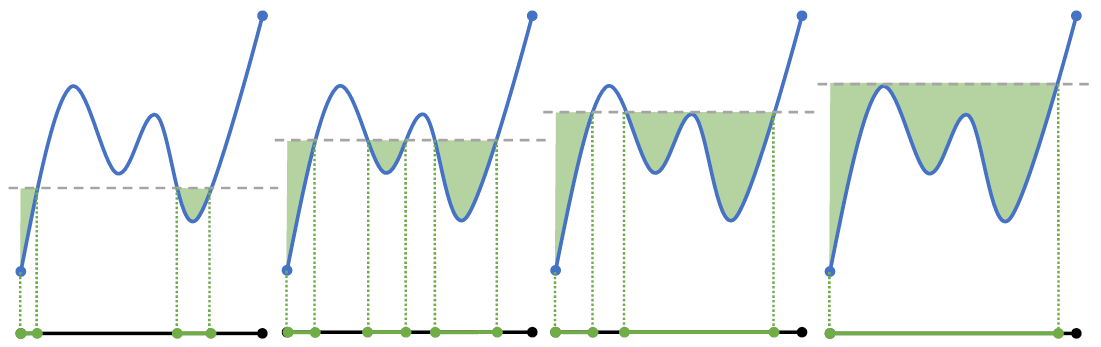
\includegraphics[width=\textwidth]{include/figuras/Sub-level Filtrations.png} 
\caption{Componentes conexas en $\mathbb{R}$ en las diferentes filtraciones. Fuente: \cite{presentacionJustin}}
\label{ref:subnivelR}
\end{figure}

Los puntos críticos de $f$ los vamos a emparejar de la siguiente forma: 
\begin{enumerate}
	\item Cuando aparece una nueva componente conexa, diremos que el mínimo local que lo crea \emph{representa} esa componente.  
	\item Cuando pasamos por un máximo local y se juntan dos componentes, emparejamos el máximo con el mayor (el más joven) de los dos mínimos locales que representan dichas componentes. El otro mínimo (el más antiguo) pasa a ser el representante de la nueva componente resultante de juntar las dos anteriores.
\end{enumerate}

Cuando los puntos $x_1$ y $x_2$ se emparejan siguiendo este método, definimos la \emph{persistencia} del par como $f(x_2) - f(x_1)$. Esta persistencia es codificada a través del \emph{diagrama de persistencia}, representando cada par con el punto $(f(x_1),f(x_2))$, como se puede ver en la figura \ref{ref:persistenciaR}. Se puede observar que todos los puntos se encontrarán por encima de la diagonal $y=x$, y que la persistencia es la distancia vertical de un punto a la diagonal. Por razones que explicaremos después se añadirán los puntos de la diagonal al diagrama de persistencia. 

\begin{figure}[!ht]
\centering
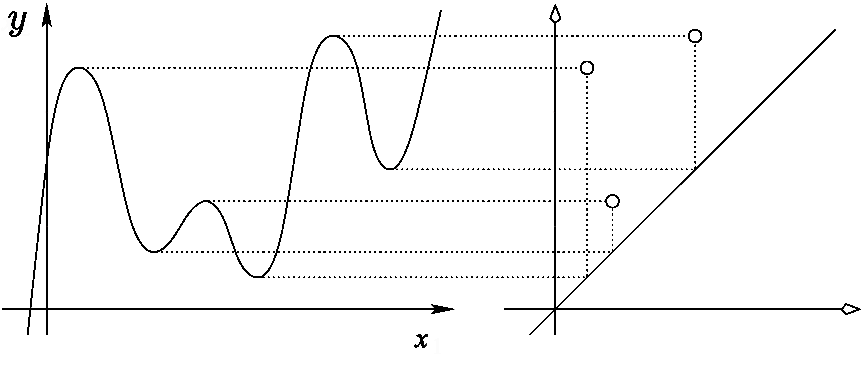
\includegraphics[width=0.8\textwidth]{include/figuras/diagramaR.png} 
\caption{Emparejamiento de los puntos críticos de la función de la función de la izquierda representados como puntos en el diagrama de persistencia de la derecha. Fuente: \cite{articuloPersistenciaEH}}
\label{ref:persistenciaR}
\end{figure}

\subsubsection*{Funciones Morse} 
Vamos a generalizar lo visto con funciones de una variable en $\mathbb{R}$ a funciones suaves sobre \emph{variedades diferenciables} con ciertas propiedades que explicaremos más adelante. Primero recordaremos que son las variedades diferenciables.

\begin{definition}
Una \emph{variedad diferenciable} un espacio topológico $\mathbb{M}$ que satisface:
\begin{enumerate}
	\item $\mathbb{M}$ es Hausdorff.
	\item $\mathbb{M}$ es segundo numerable.
	\item Todo punto de $\mathbb{M}$ posee un entorno homomorfo a $\mathbb{R}^n$.
	\item Todo punto de $\mathbb{M}$ posee un entorno abierto difeomorfo a $\mathbb{R}^n$.
\end{enumerate}
\end{definition}

Sea $f: \mathbb{M} \longrightarrow \mathbb{R}$ una aplicación diferenciable ($C^\infty$). En este caso, un \emph{punto crítico} es un punto $p \in \mathbb{M}$ tal que $\dfrac{\partial f}{\partial x_i}(p)=0$ para $i = 1, ..., n$. Un punto crítico $p$ es \emph{no degenerado} si la matriz Hessiana de las segundas derivadas parciales,
\[
(H_f)_{i,j}=\dfrac{\partial^2 f}{\partial x_i \partial x_j}
\]
es no singular. Si $p$ es un punto crítico no degenerado se define su \emph{índice} como el número de autovalores negativos de la matriz Hessiana en $p$.

\begin{figure}[!ht]
\centering
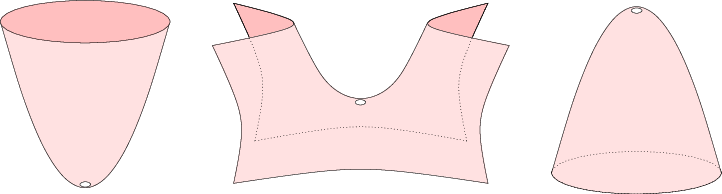
\includegraphics[width=0.7\textwidth]{include/figuras/From-left-to-right-a-minimum-saddle-and-maximum-of-the-vertical-height-function.png} 
\caption{De izquiera a derecha tenemos: un punto crítico no degenerado de índice 0, 1 y 2. Fuente: \cite{articuloPersistenciaEH}}
\label{ref:morseCriticos}
\end{figure}

\begin{definition}
Sea $f: \mathbb{M} \longrightarrow \mathbb{R}$ una aplicación diferenciable. Diremos que $f$ es una \emph{función Morse} si todos sus puntos críticos son no degenerados y tienen distintos valores críticos.
\end{definition}

\begin{sloppypar}
Se puede demostrar que las funciones Morse poseen un número finito de puntos críticos. Elegimos los valores regulares $t_0 < t_1 < ... < t_m$ tal que ${\exists!\ p_i \in (t_i, t_{i+1})}$ punto crítico para todo $i = 0, ..., m-1$. Sea $\mathbb{M}_j=f^{-1}(-\infty, t_j]$ el \emph{conjunto de subnivel} que contiene los primeros $j$ puntos críticos.
\end{sloppypar}

Cuando pasamos de $\mathbb{M}_{j-1}$ a $\mathbb{M}_j$ la homología puede cambiar de dos formas distintas:
\begin{enumerate}[label=\Alph*)]
	\item $H_p$ incrementa la dimensión en uno, es decir, ${\beta_p(\mathbb{M}_j)} = \beta_p(\mathbb{M}_{j-1} + 1)$.
	\item $H_{p-1}$ disminuye la dimensión en uno, es decir, ${\beta_{p-1}(\mathbb{M}_j)} = \beta_{p-1}(\mathbb{M}_{j-1} - 1)$.
\end{enumerate}
Donde $p$ es el índice del $j$-ésimo punto crítico. En el primer caso denotaremos a ese punto crítico como \emph{punto crítico positivo} y en el segundo como \emph{punto crítico negativo}.

\subsubsection*{funciones tame}
definición función tame, subniveles, grupos de persistencia a partir de funciones tame, critical value lema,  números de betti de grupos de persistencia y su relación con las multiplicidades.

Definición de diagrama de persistencia, k-triangle lemma


\subsubsection*{persistencia en complejos simpliciales}
particularizar lo visto en funciones tame pero con complejos simpliciales

\subsubsection*{funciones PL}
definición de las funciones pl, generación de filtraciones a partir del lower star filtration y estudio de los puntos críticos  de las funciones pl para comprobar que son funciones tame.



